\section{Per-round Self-attribution Breakdown}
\label{sec:appendix:self-attribution}

This appendix expands the aggregate self-attribution result of \S\ref{sec:experiments:rq3b} with a per-round breakdown across the four fix/regression by precision/recall panels.

\Cref{fig:pred-fix,fig:pred-reg} show the per-round breakdown across the four fix/regression by precision/recall panels. Bars decompose each denominator, predicted for precision and actual for recall, into deep-blue TP versus pale FP or FN; the dashed line traces the metric on the right-hand $0$ to $100\%$ axis, and the solid line shows contemporaneous pass@1. Fix-precision and fix-recall both swing from near-zero to near-saturation across rounds, so the evolve model's causal attribution for its own improvements is informative if noisy. Regression predictions instead stay near the floor, below $25\%$ on most rounds: across the 9 rounds the agent issued 43 unique regression predictions and only 5 landed, giving cumulative $P=11.6\%$, while 40 regressions the agent did not foresee actually occurred, giving cumulative $R=11.1\%$.

\begin{figure}[t]
    \centering
    \begin{minipage}{0.49\linewidth}
        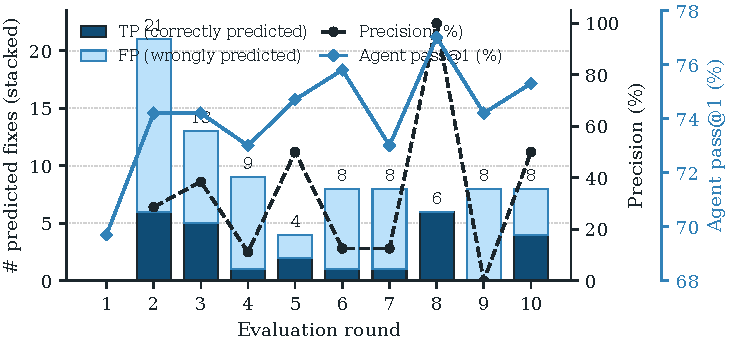
\includegraphics[width=\linewidth]{figures/prediction_fix_precision.pdf}
    \end{minipage}
    \hfill
    \begin{minipage}{0.49\linewidth}
        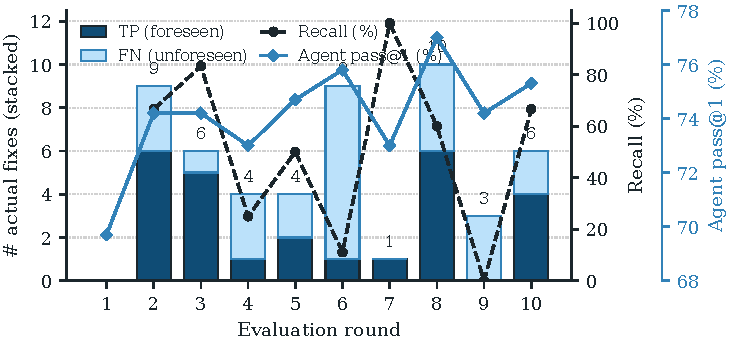
\includegraphics[width=\linewidth]{figures/prediction_fix_recall.pdf}
    \end{minipage}
    \caption{Per-round fix predictions. Left: precision. Right: recall. Bars decompose each denominator into TP versus FP or FN; lines overlay the metric and contemporaneous pass@1.}
    \label{fig:pred-fix}
\end{figure}

\begin{figure}[t]
    \centering
    \begin{minipage}{0.49\linewidth}
        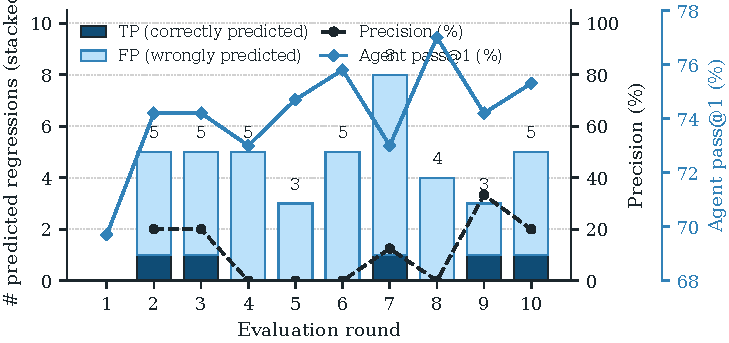
\includegraphics[width=\linewidth]{figures/prediction_regression_precision.pdf}
    \end{minipage}
    \hfill
    \begin{minipage}{0.49\linewidth}
        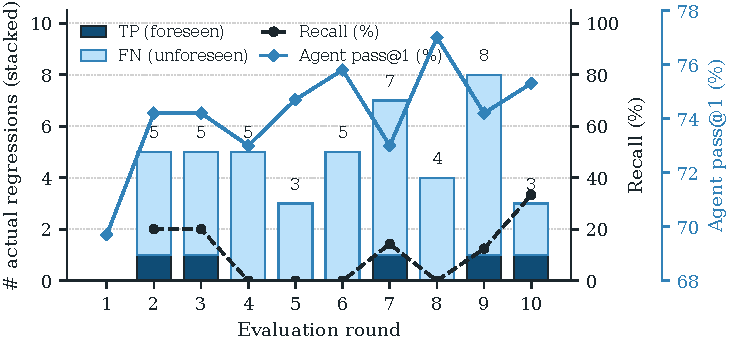
\includegraphics[width=\linewidth]{figures/prediction_regression_recall.pdf}
    \end{minipage}
    \caption{Per-round regression predictions. Left: precision. Right: recall. Same encoding as Fig.~\ref{fig:pred-fix}.}
    \label{fig:pred-reg}
\end{figure}
